\documentclass[12pt, a4paper]{article}
\usepackage[utf8]{inputenc}

\title{Control of robotic arm and gripper}
\author{Cristian Enrico Capalbo}
\date{\today}
\usepackage{graphicx}
\usepackage{wrapfig}
\usepackage{subcaption}
\graphicspath{ {images/} }

\begin{document}

\maketitle
\newpage

\section{Introduction}
In the original design of the robot, the degrees of freedom of the arm and the gripper (the end effector) are controlled by means of a remote controller. 

\begin{figure}[ht]
	\begin{minipage}[b]{0.45\linewidth}
		\centering
		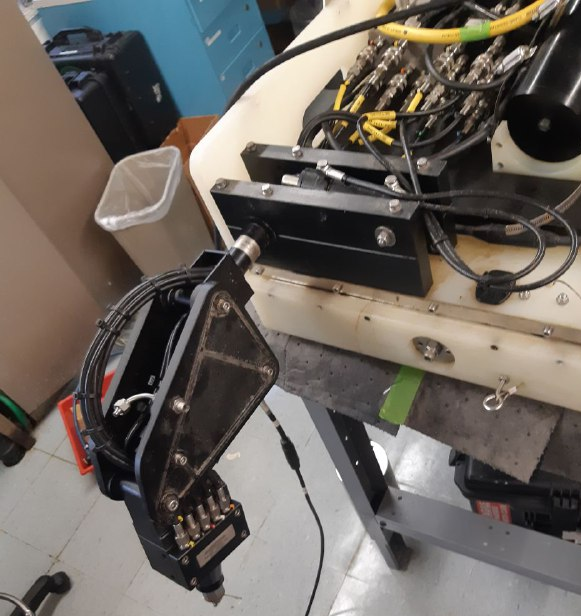
\includegraphics[width=\textwidth]{arm}
		\caption{Robotic arm}
		\label{fig:arm}
	\end{minipage}
	\hspace{0.5cm}
	\begin{minipage}[b]{0.45\linewidth}
		\centering
		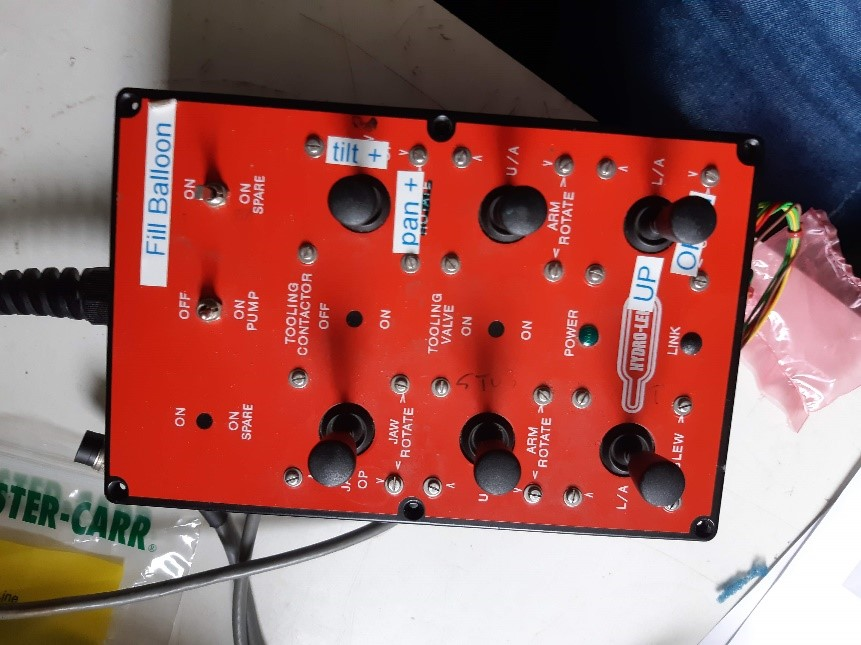
\includegraphics[width=\textwidth, angle=-90]{remote.jpg}
		\caption{Remote controller}
		\label{fig:remote}
	\end{minipage}
\end{figure}

Although this is the best solution, as it was at the start of the experience it showed a sort of a lag, since there was a delay between the moment in which the command was sent and the effective movement; also, if the command was too short the arm didn’t move at all. 
\\
At the starting point the reason of this problem was unknown, it could either be the control electronics or the hydraulic actuation of the system. We choose to examine first the electronics, then go on with the hydraulic valves if necessary.
\\ 

\section{Electronics}
The electronic system consists initially of a printed board, housed in the remote, to which all the cables from the several joysticks are connected. This board reads the analogic signals and sends them to the on-board controller of the valves through an ethernet connection. The printed board contains some chips that could cause the delay, and each of them has been analysed.
\newpage\subsection{Multiplexer}
The first element analysed is a Multiplexer (TI CD74HC151E); in the board we can see three of them, each connected to the outputs of two joysticks. The function of the multiplexer is to read the 8 signals in input and giving as an output a single signal. To check if the delay was introduced in the system by this component we didn’t need to know exactly how it works; what we did is simply connecting the output port of the multiplexer to an oscilloscope and verify that the change in the output happened instantly after the movement of the joystick. Being this verified we passed to the next element.

\begin{figure}[h]
	\begin{subfigure}[t]{0.4\textwidth}
		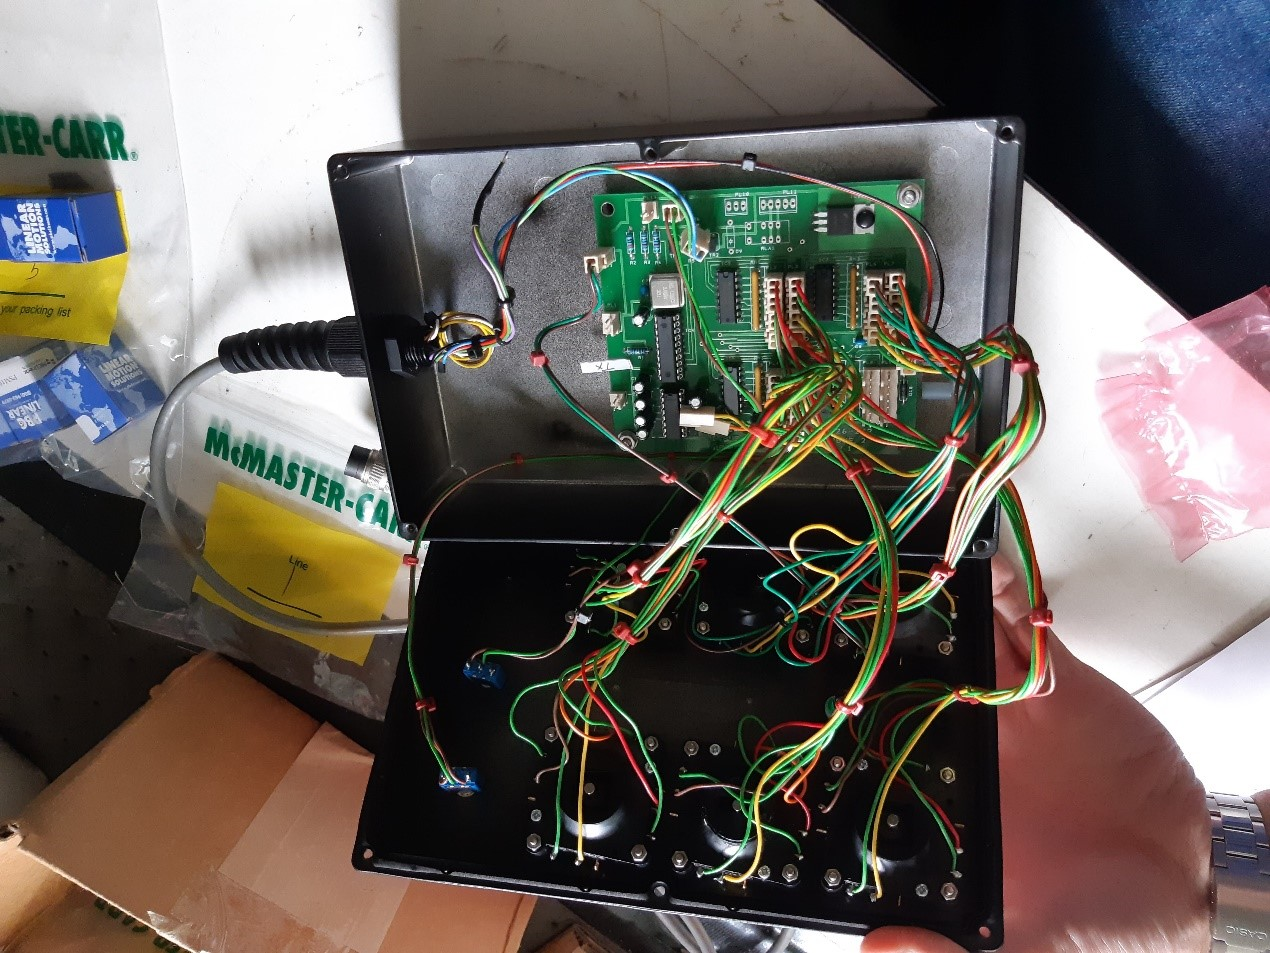
\includegraphics[width=\textwidth]{remote_internal} 
		\caption{Internal parts of the remote}
		\label{fig:remote_in}
	\end{subfigure}
	\hfill%
	\begin{subfigure}[t]{0.4\textwidth}
		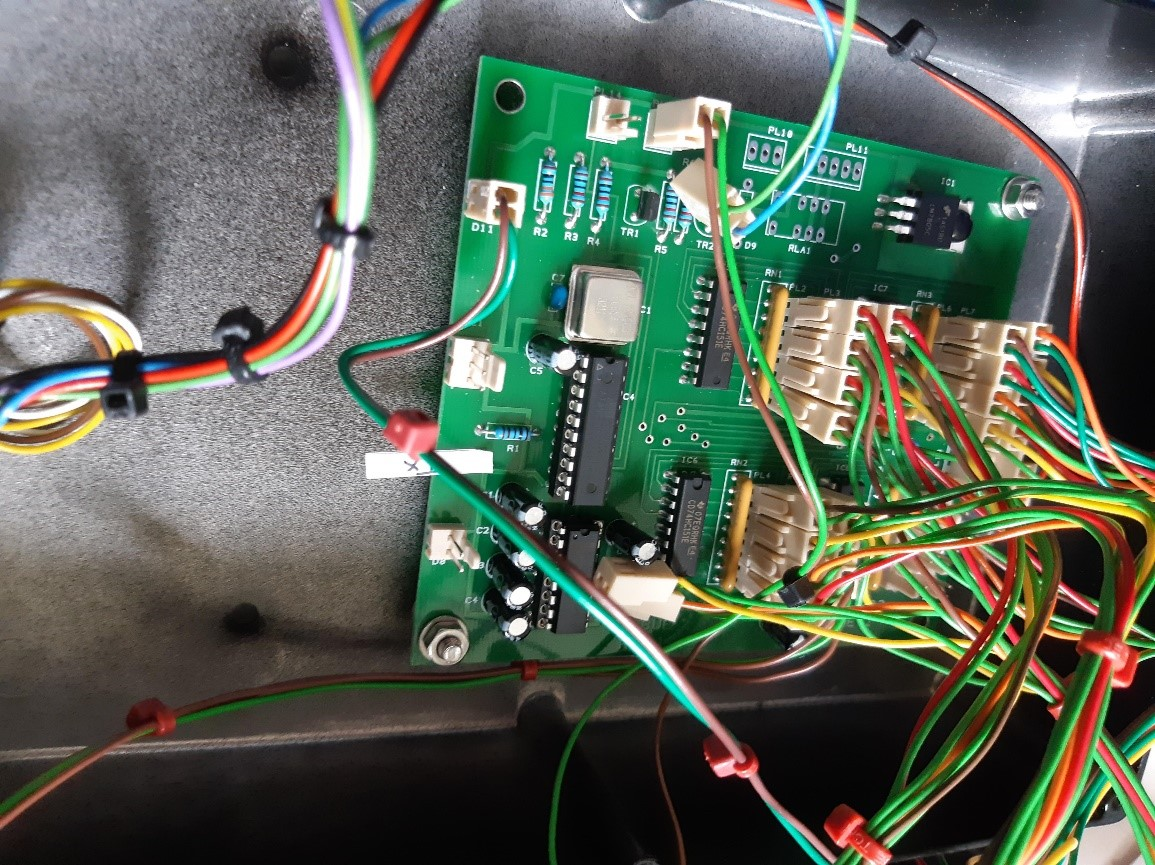
\includegraphics[width=\textwidth]{remote_board}
		\caption{Electrical board of the remote}
		\label{fig:remote_board}
	\end{subfigure}
 	\caption{Components of the remote}
	\label{fig:remote_comps}
\end{figure}

\begin{figure}[h]
	\begin{subfigure}[t]{0.4\textwidth}
		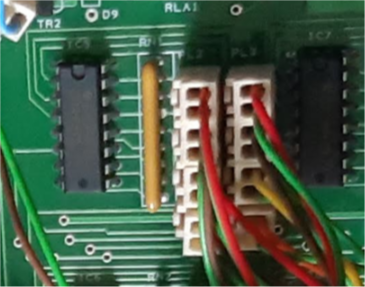
\includegraphics[width=\textwidth]{remote_multiplexer} 
		\caption{Multiplexer (TI CD74HC151E)}
		\label{fig:multiplexer}
	\end{subfigure}
	\hfill%
	\begin{subfigure}[t]{0.2\textwidth}
		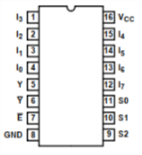
\includegraphics[width=\textwidth]{multiplexer_ports}
		\caption{Multiplexer ports configuration}
		\label{fig:rmultiplexer_ports}
	\end{subfigure}
	\hfill%
	\begin{subfigure}[t]{0.2\textwidth}
		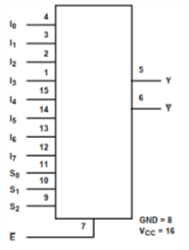
\includegraphics[width=\textwidth]{multiplexer_scheme}
		\caption{Multiplexer functioning scheme}
		\label{fig:multiplexer_scheme}
	\end{subfigure}
 	\caption{Multiplexer}
	\label{fig:multi}
\end{figure}
\newpage\subsection{Microcontroller}

The second element analysed, connected right after the three multiplexers, is an 8-bit microcontroller (ATMEL AT89C2051). As in the precedent case, we didn’t need to know the actual functioning logic behind this component; all we needed to know is what was the output. From the connection to the other elements of the board we understood that it gave as output a serial signal in TTL/COMS format. To inspect this signal the output port was connected to an Mbed platform in turn connected to a computer through an USB port. A simple code was loaded in the platform that permitted to read the serial data from the microcontroller output and sent it to the computer; on this last one a software read and printed the messages. In this way we could see that the microcontroller maps every configuration of the joystick in a single Comma Separated Values string whit 5 numbers of 2 digits each. We could also see that there’s no delay in this signal.

\begin{figure}[ht]
	\begin{minipage}[b]{0.45\linewidth}
		\centering
		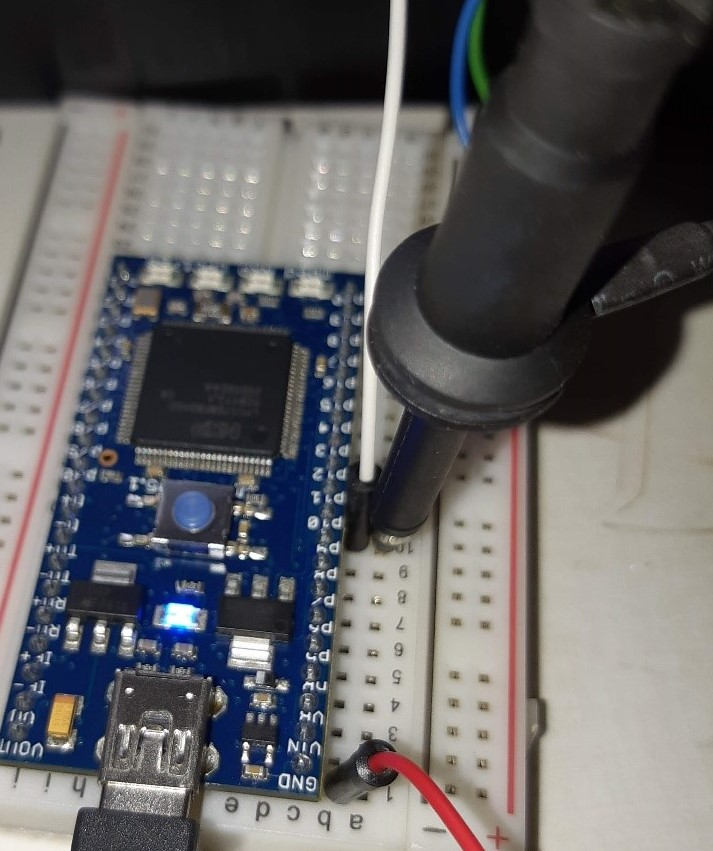
\includegraphics[width=\textwidth]{mbed}
		\caption{mbed configuration}
		\label{fig:mbed}
	\end{minipage}
	\hfill%
	%\hspace{0.5cm}
	\begin{minipage}[b]{0.45\linewidth}
		\centering
		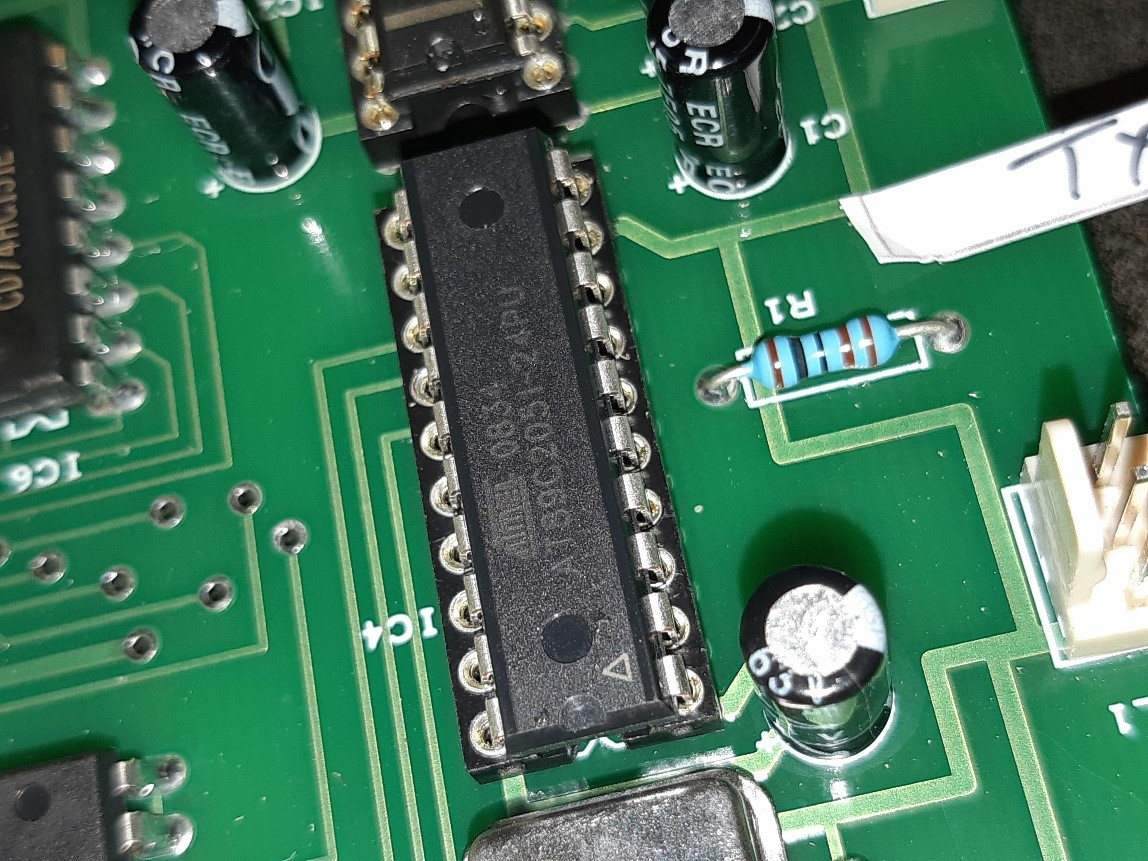
\includegraphics[width=\textwidth, angle=-90]{microcontroller}
		\caption{microcontroller (ATMEL AT89C2051)}
		\label{fig:microcontroller}
	\end{minipage}
\end{figure}
\subsection{RS232 driver}	
The last element in the remote electronics is a driver (MAX232) that has the only function of a communication interface between TTL/CMOS and RS232 standard that is the one used as output to communicate with the electronics on the ROV. Since it has multiple channels to actuate the translation in both ways, we took the first output (RS232) and translated it again in TTL/CMOS in order to read it with the same Mbed system. Also in this case we couldn’t see any delay, so the next step was to examine the onboard electronics. 

\begin{figure}[h]
	\begin{subfigure}[t]{0.4\textwidth}
		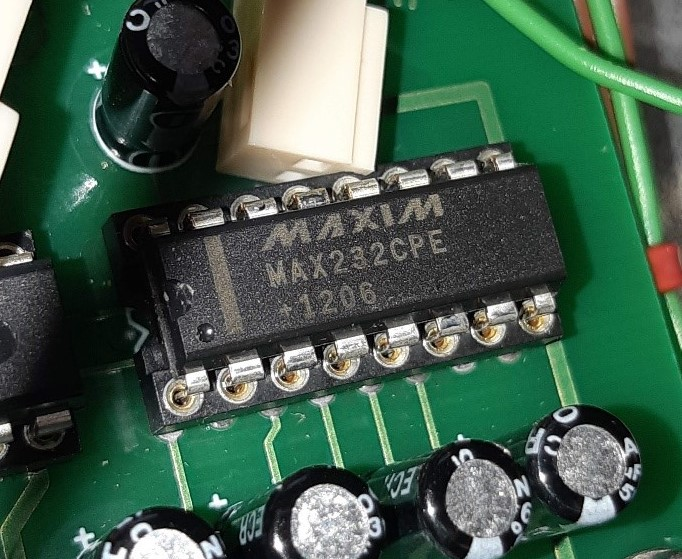
\includegraphics[width=\textwidth]{max232} 
		\caption{MAXIM MAX232CPE}
		\label{fig:max232}
	\end{subfigure}
	\hfill%
	\begin{subfigure}[t]{0.4\textwidth}
		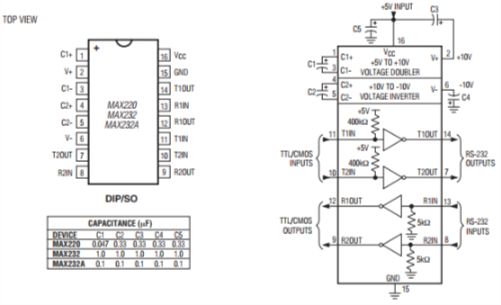
\includegraphics[width=\textwidth]{max232_scheme}
		\caption{max232 functioning scheme}
		\label{fig:max232_scheme}
	\end{subfigure}
 	\caption{MAX232}
	\label{fig:max}
\end{figure}

\end{document}